\documentclass[10pt]{beamer}

\usetheme{metropolis}
\usepackage{appendixnumberbeamer}

\usepackage{booktabs}
\usepackage{multirow}
\usepackage[scale=2]{ccicons}

\usepackage{pgfplots}
\usepgfplotslibrary{dateplot}

\usepackage{xspace}
\usepackage{xcolor}
\newcommand{\themename}{\textbf{\textsc{metropolis}}\xspace}
\usepackage{tabularx}

\usepackage[utf8]{inputenc}
\usepackage[brazilian]{babel}

\usepackage{blindtext}
\usepackage[portuguese, noend, plain, linesnumbered]{algorithm2e}

\setbeamercolor{background canvas}{bg=white}

\title{}
\subtitle{Uso de Redes de Função de Base Radial e Cadeias de Markov para detecção online de mudanças de conceito em fluxos contínuos de dados}
\date{}
\author{\textbf{Discente:} Ruivaldo Neto \newline \textbf{Orientador:} Ricardo Rios}
\institute{Universidade Federal da Bahia \newline Departamento de Ciência da Computação \newline Programa de Pós-Graduação em Ciência da Computação \newline\newline Contato: rneto@rneto.dev \newline\newline 16 de Dezembro de 2019}

\titlegraphic{%
  \begin{picture}(0,0)
    \put(330, 28){\makebox(0,0)[rt]{
\includegraphics[scale=0.25]{logo.png}}}
  \end{picture}
}

\begin{document}

\maketitle

\begin{frame}{Roteiro}
  \setbeamertemplate{section in toc}[sections numbered]
  \begin{minipage}{\textwidth}
    \tableofcontents
  \end{minipage}
\end{frame}

\section{Introdução}

\begin{frame}{Introdução}
    \begin{itemize}
        \item<1 -> Avanços tecnológicos recentes contribuiram para o aumento do volume de dados produzidos por sistemas computacionais \cite{idc_report}.
        \item<1 -> Parte significativa desse volume é produzida na forma de \alert{Fluxos Contínuos de Dados (FCDs)}: sequências \alert{ininterruptas} e \alert{potencialmente infinitas} de eventos \cite{Aggarwal:2006:DSM:1196418}.
        \item<1 -> FCDs estão presentes em variados domínios de aplicação:
        \begin{itemize}
            \item Análise do Mercado Financeiro;
            \item Gestão de redes de telecomunicação;
            \item Detecção de intrusos;
            \item Monitoramento de tráfico; etc.
        \end{itemize}
      \end{itemize}
\end{frame}

\begin{frame}{Introdução}
    \begin{itemize}
        \item<1 -> Técnicas de \alert{Aprendizado de Máquina (AM)} são utilizadas para extrair informações úteis desses grandes conjuntos de dados.
        \item<1 -> Cenários com FCDs limitam a aplicação dessas técnicas, pois impõem restrições de tempo de resposta, de uso dos recursos computacionais e apresentam comportamento \alert{não estacionário}.
        \item<1 -> Em cenários \alert{não estacionários}, o contexto do processo gerador e/ou a distribuição dos dados podem sofrer alterações ao longo do tempo.
        \item<1 -> Essas mudanças, denominadas \alert{mudanças de conceito} (\textit{concept drifts}), podem ter impacto negativo nas técnicas de AM aplicadas.
      \end{itemize}
\end{frame}

\begin{frame}{Introdução}
    \begin{itemize}
        \item<1 -> Inicialmente, realizava-se a atualização periódica dos modelos para mitigar os efeitos das mudanças de conceito.
        \item<1 -> Pesquisadores propuseram métodos mais precisos e eficazes baseados em monitoramento.
        \item<1 -> Os métodos propostos apresentam limitações ao serem aplicados em cenários com FCDs \cite{Aggarwal:2006:DSM:1196418}:
        \begin{itemize}
            \item<1 -> Necessidade de rotulação;
            \item<1 -> Não atendem às restrições (tempo de resposta e uso de recursos).
        \end{itemize}
      \end{itemize}
\end{frame}

\begin{frame}{Introdução}
    \begin{itemize}
        \item<1 -> Visando superar essas limitações, este trabalho propõe um novo método de detecção de mudanças de conceito baseado em \alert{Redes de Função de Base Radial (redes RBF) e Cadeias de Markov}, denominado \textbf{\alert{RBFChain}}.
        \item<1 -> O método proposto se diferencia por detectar mudanças em \alert{tempo de execução}, de forma computacionalmente \alert{eficiente} e \alert{independente de rótulos}.
    \end{itemize}
\end{frame}

\section{Fundamentação Teórica}

\begin{frame}{Fluxos Contínuos de Dados e Aprendizado de Máquina}
    \begin{itemize}
        \item<1 -> \alert{Fluxos Contínuos de Dados (FCDs)} são sequências ininterruptas e potencialmente infinitas de eventos \cite{Aggarwal:2006:DSM:1196418}, que não podem ser armazenados e devem ser analisados em tempo de execução.
        \item<1 -> Algoritmos de AM foram adaptados para atender a essas restrições \cite{Aggarwal:2003:FCE:1315451.1315460}, mas ainda são sucetíveis a \alert{mudanças de conceito}.
      \end{itemize}
\end{frame}

\begin{frame}{Mudança de Conceito}
    \begin{itemize}
        \item<1 -> \alert{Mudanças de conceito} são alterações no contexto do processo e/ou na distribuição dos dados que podem impactar negativamente técnicas de AM.
        \item<1 -> Podem ser definidas formalmente através da Teoria Bayesiana de Decisão \cite{Duda:2000:PC:954544}: sendo $p_{t_0}$ e $p_{t_1}$ as distribuições de probabilidades conjuntas nos instantes $t_0$ e $t_1$, há mudança de conceito entre $t_0$ e $t_1$ se:
        \begin{equation} \label{eq:3}
            {\exists}X : p_{t_0}(X, c) \ne p_{t_1}(X, c)
        \end{equation}
        % \item<1 -> $X$ possui uma classificação legítima em $t_0$, mas passa a ter outra, também legítima, em $t_1$.
    \end{itemize}
\end{frame}

\begin{frame}{Mudança de Conceito}
    \begin{itemize}
        \item<1 -> São categorizadas como \alert{Virtuais} ou \alert{Reais} \cite{Gama:2014:SCD:2597757.2523813}:
        \begin{itemize}
        \item<1 -> \alert{Mudanças Virtuais} são alterações na probabilidade a priori das classes, $P(c)$, e \alert{\textbf{não modificam} os resultados esperados}.
        \item<1 -> \alert{Mudanças Reais} são alterações na probabilidade a posteriori, $p(c|X)$, e \alert{\textbf{modificam} os resultados esperados}.
        \end{itemize}
    \end{itemize}
\end{frame}

\begin{frame}{Mudança de Conceito}
\begin{figure}[H]
    \begin{center}
        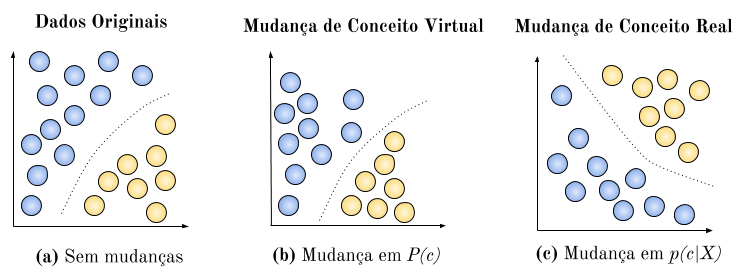
\includegraphics[scale=0.55]{imagens/concept_drift.png}
        \caption{Mudança de Conceito Virtual vs. Mudança de Conceito Real.}
        \label{fig:real_and_virtual_concept_drift}
    \end{center}
\end{figure}
\end{frame}

\begin{frame}{Mudança de Conceito}
    \begin{itemize}
        \item<1 -> Ocorrem de forma \alert{abrupta}, \alert{gradual}, \alert{incremental} ou \alert{recorrente} \cite{Zliobaite:2010}.
    \end{itemize}
    \begin{figure}[H]
        \begin{center}
            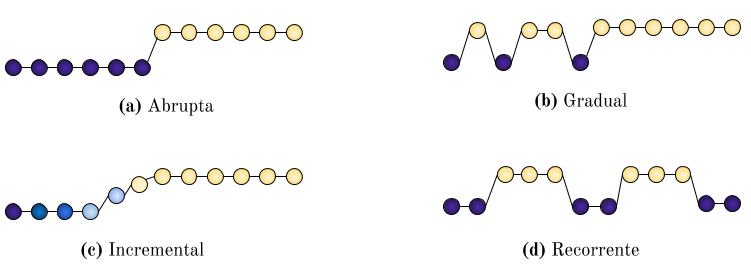
\includegraphics[scale=0.55]{imagens/concept_drift_patterns.png}
            \caption{Padrões de ocorrência de Mudanças de Conceito.}
            \label{fig:concept_drift_patterns}
        \end{center}
    \end{figure}
\end{frame}

\begin{frame}{Algoritmos para Detecção de Mudança de Conceito}
    \begin{itemize}
        \item<1 -> Algoritmos de detecção se dividem em dois grupos, conforme a necessidade de rotulação dos dados \cite{Zliobaite:2010}:
        \begin{itemize}
        \item<1 -> \alert{Explícitos/Supervisionados}: \textbf{Dependem} da rotulação dos dados. Realizam a detecção a partir do monitoramento de medidas de performance como taxa de erro e acurácia.
        \item<1 -> \alert{Implícitos/Não Supervisionados}: \textbf{Independem} da rotulação dos dados. Realizam a detecção através do monitoramento de características dos próprios dados ou de indicadores produzidos pelas técnicas de aprendizado aplicadas.
        \end{itemize}
    \end{itemize}
\end{frame}

\begin{frame}{Ferramenta: MOA}
    \begin{itemize}
        \item<1 -> O MOA é o principal framework para pesquisa com fluxos contínuos.
        \item<1 -> Possui rotinas para produzir dados sintéticos e para avaliar métodos de detecção de mudança de conceito.
    \end{itemize}
    \begin{figure}[H]
        \begin{center}
            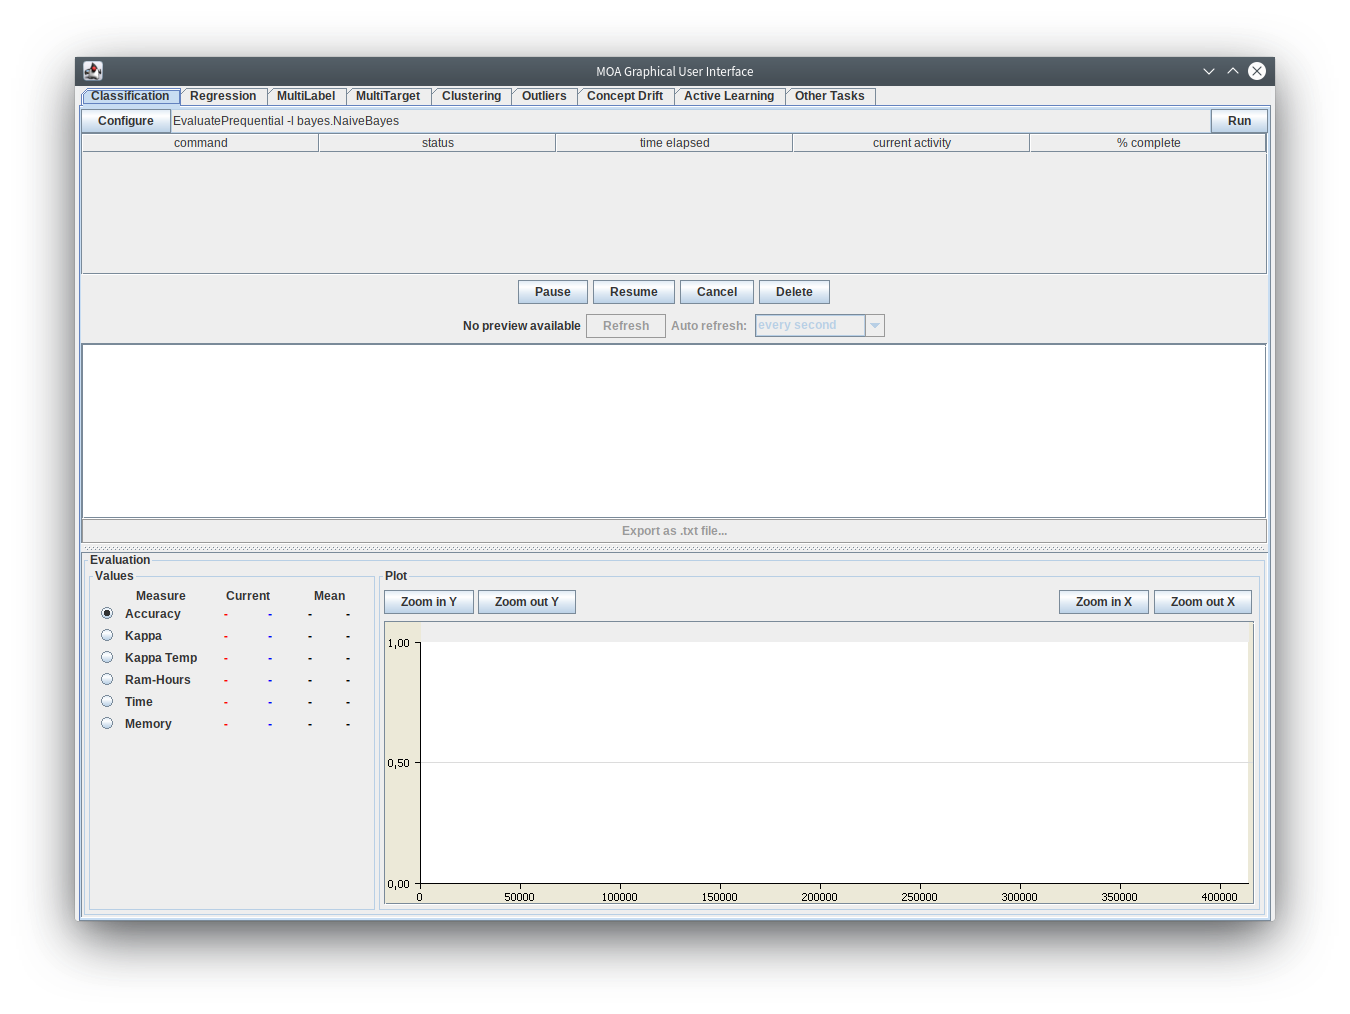
\includegraphics[scale=0.18]{imagens/moa.png}
            \caption{MOA - Tela Inicial.}
            \label{fig:moa}
        \end{center}
    \end{figure}
\end{frame}

\begin{frame}{Mudança de Conceito - RBFChain}
    \begin{itemize}
        \item<1 -> O método proposto identifica mudanças \alert{sob qualquer padrão de ocorrência}.
        \item<1 -> É independente de rótulos, logo considera todas mudanças identificadas como \alert{mudanças reais}.
        \item<1 -> Foi implementado e validado através do MOA.
    \end{itemize}
\end{frame}

\begin{frame}{Redes de Função de Base Radial}
    \begin{itemize}
        \item<1 -> \alert{Redes de Função de Base Radial} são redes neurais cuja ativação é realizada através do cálculo da distância entre o evento e um centro definido \cite{Braga:RedesNeuraisTeoriaAplicacoes}.
        \item<1 -> A arquitetura mais básica para redes RBF envolve três camadas:
        \begin{itemize}
            \item<1 -> \alert{Entrada}: Recepciona os dados e encaminha para camada intermediária.
            \item<1 -> \alert{Intermediária}: Composta por funções de ativação de base radial que atuam como neurônios.
            \item<1 -> \alert{Saída}: Pondera os resultados da camada intermediária, agregando-os linearmente para compor a resposta final da rede.
        \end{itemize}
        % \item<1 -> Na literatura, as funções Gaussianas são as funções de ativação mais empregadas em redes RBF.
      \end{itemize}
\end{frame}

\begin{frame}{Redes de Função de Base Radial}
    \begin{figure}[H]
    \begin{center}
        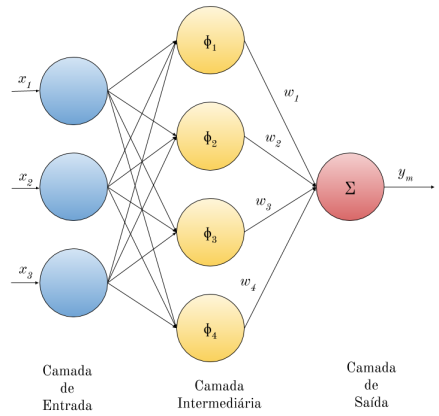
\includegraphics[scale=0.63]{imagens/rbf_arq.png}
        \caption{Arquitetura RBF.}
        \label{fig:rbg_arq}
    \end{center}
    \end{figure}
\end{frame}

\begin{frame}{Redes de Função de Base Radial}
    \begin{itemize}
        \item<1 -> O RBFChain utiliza uma rede RBF adaptada, composta apenas pelas camadas inicial e intermediária.
        \item<1 -> O processo de ativação da camada intermediária produz, implicitamente, grupos dos eventos recebidos.
        \item<1 -> Mudanças de conceito são identificadas quando o grupo ativo desse agrupamento é alterado.
      \end{itemize}
\end{frame}


% \begin{frame}{Cadeias de Markov}
%     \begin{itemize}
%         \item<1 -> Equações determinísticas não podem ser utilizadas para descrever sistemas com múltiplos caminhos evolutivos;
%         \item<1 -> Nestes casos, \alert{processos estocásticos} são utilizados \cite{taylor1998introduction};
%         \item<1 -> Um \alert{processo estocástico} é uma coleção de variáveis aleatórias indexadas no tempo: $\left\{ X _ { t } : t \in T \right\}$;
%         \item<1 -> Considerando que o processo estocástico esteja no estado $s_i$ e no tempo $t - 1$, a probabilidade
%         do processo estar no estado $s_j$ no tempo $t$ é dada pela Equação \ref{eq:prob_proc_estoc}:
%         \begin{equation}
%             \label{eq:prob_proc_estoc}
%             \mathbb { P } \left( X _ { t } = s _ { j } | X _ { t - 1 } = s _ { i } , \ldots , X _ { 0 } = s _ { 0 } \right)
%         \end{equation}
%       \end{itemize}
% \end{frame}

\begin{frame}{Cadeias de Markov}
    \begin{itemize}
        \item<1 -> \alert{Cadeias de Markov} são processos estocásticos no qual a probabilidade do estado em um determinado período de tempo depende apenas do estado no período imediatamente anterior (Equação \ref{eq:markov}).
        \begin{equation}
            \label{eq:markov}
            \mathbb { P } \left( X _ { t } = s _ { j } | X _ { t - 1 } = s _ { i } , \ldots , X _ { 0 } = s _ { 0 } \right) = \mathbb { P } \left( X _ { t } = s _ { j } | X _ { t - 1 } = s _ { i } \right) = p _ { i j }
        \end{equation}
      \end{itemize}
\end{frame}

\begin{frame}{Cadeias de Markov}
    \begin{itemize}
        \item<1 -> A Cadeia de Markov pode assumir os estados $a_1, a_2, \ldots, a_r$, de tal modo que a probabilidade de transição de um estado $a_i$ para um estado $a_j$ seja $P_{ij}$ (um valor dependente apenas de $i$ e $j$);
        \item<1 -> As probabilidades entre estados podem ser representadas por uma matriz estocástica (Equação \ref{eq:matriz_estocastica}):
        \begin{equation}
            \label{eq:matriz_estocastica}
            P = \left[ \begin{array} { c c c c } { P _ { 11 } } & { P _ { 12 } } & { \dots } & { P _ { 1 r } } \\ { P _ { 21 } } & { P _ { 22 } } & { \dots } & { P _ { 2 r } } \\ { \vdots } & { \vdots } & { \vdots } & { \vdots } \\ { P _ { r 1 } } & { P _ { r 2 } } & { \cdots } & { P _ { r r } } \end{array} \right]
        \end{equation}
      \end{itemize}
\end{frame}

\begin{frame}{Cadeias de Markov}
    \begin{figure}[H]
        \begin{center}
            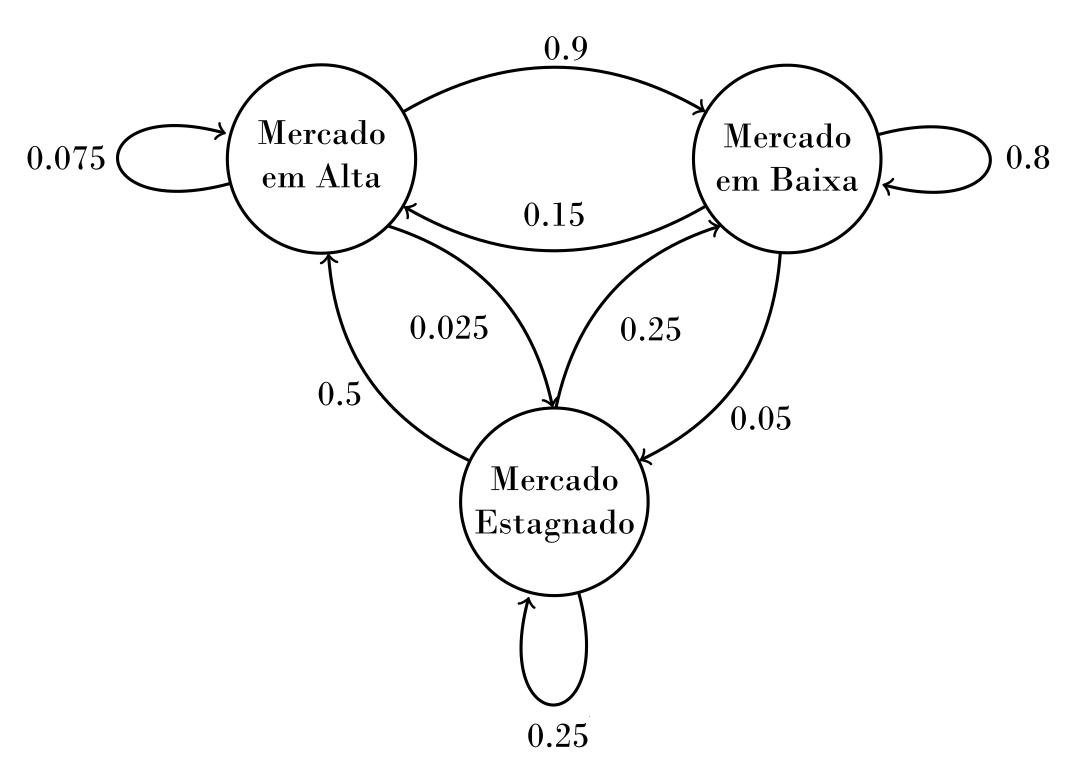
\includegraphics[scale=0.23]{imagens/markov_chain_wikipedia.png}
            \caption{Representação Gráfica: Cadeia de Markov com três estados.}
            \label{fig:cadeia_markov_tres_estados}
        \end{center}
    \end{figure}
\end{frame}

\begin{frame}{Cadeias de Markov}
    \begin{itemize}
        \item<1 -> O RBFChain utiliza uma Cadeia de Markov para modelar o agrupamento criado na rede RBF adaptada.
        \item<1 -> Os grupos formados representam os estados e as ativações de novos grupos, as transições.
        \item<1 -> As transições são refletidas no modelo markoviano através do aumento da probabilidade correspondente e a diminuição proporcional das outras transições, respeitando a condição: $0 \leq P_{ij} \leq 1$.
      \end{itemize}
\end{frame}

\begin{frame}{Trabalhos Relacionados}
    \begin{itemize}
        \item<1 -> Pesquisa na literatura em busca de trabalhos que propõem métodos para identificação de mudanças de conceito em fluxos contínuos de dados, de forma online e independente de rótulos.
        \item<1 -> Também foram estudadas técnicas que pudessem subsidiar o desenvolvimento de novos algoritmos que atendam a esses requisitos.
    \end{itemize}
\end{frame}

\begin{frame}{Trabalhos Relacionados}
    \begin{itemize}
        \item<1 -> Análise dos algoritmos \alert{Implícitos/Não Supervisionados} da subcategoria \alert{Detecção de Novidade / Métodos de Agrupamento}.
        \item<1 -> Análise dos métodos para detecção de \textit{Change Points} em séries temporais que atuam de forma online:
        \begin{itemize}
            \item<1 -> Modelos autoregressivos;
            \item<1 -> Séries com autosimilaridade e periodicidade.
        \end{itemize}
        \item<1 -> Análise da aplicação de algoritmos de agrupamento estáveis.
        \item<1 -> Identificação de lacuna de pesquisa.
      \end{itemize}
\end{frame}

\section{RBFChain}

\begin{frame}{Visão Geral}
    \begin{itemize}
        \item<1 -> O RBFChain atua diretamente sobre o fluxo de dados e é composto por dois componentes principais: uma Rede de Função de Base Radial (RBF) adaptada e uma Cadeia de Markov.
      \end{itemize}
\end{frame}

\begin{frame}{Visão Geral}
        \begin{figure}[H]
            \begin{center}
                
\includegraphics[scale=0.4]{imagens/arquitetura_rbfchain.png}
                \caption{Arquitetura RBFChain.}
                \label{fig:arquitetura}
            \end{center}
        \end{figure}
\end{frame}


\begin{frame}{Execução de exemplo}
    \begin{itemize}
        \item $S = {0.11, 0.12, 0.13, 0.33, 0.34, 0.45, 0.6, 0.33, 0.25, 0.14, 0.11, 0.15}$
        \item $\sigma = 3, \lambda = 0.8, \alpha = 0.25, \delta = 0.5$
    \end{itemize}
    \begin{figure}[H]
        \begin{center}
            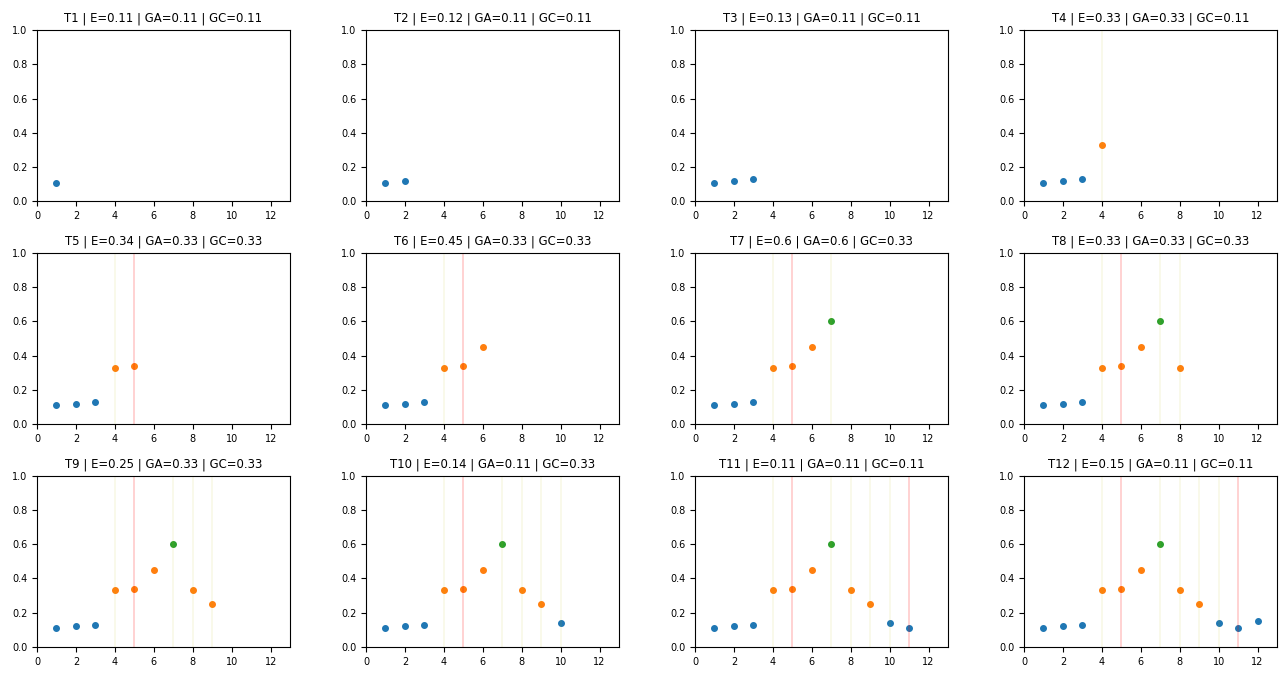
\includegraphics[width=\textwidth]{imagens/funcionamento_algoritmo.png}
            \caption{Execução de exemplo do RBFChain.}
            \label{fig:funcionamento_algoritmo}
        \end{center}
    \end{figure}
\end{frame}

\begin{frame}{Execução de exemplo}
    \begin{figure}[H]
        \begin{center}
            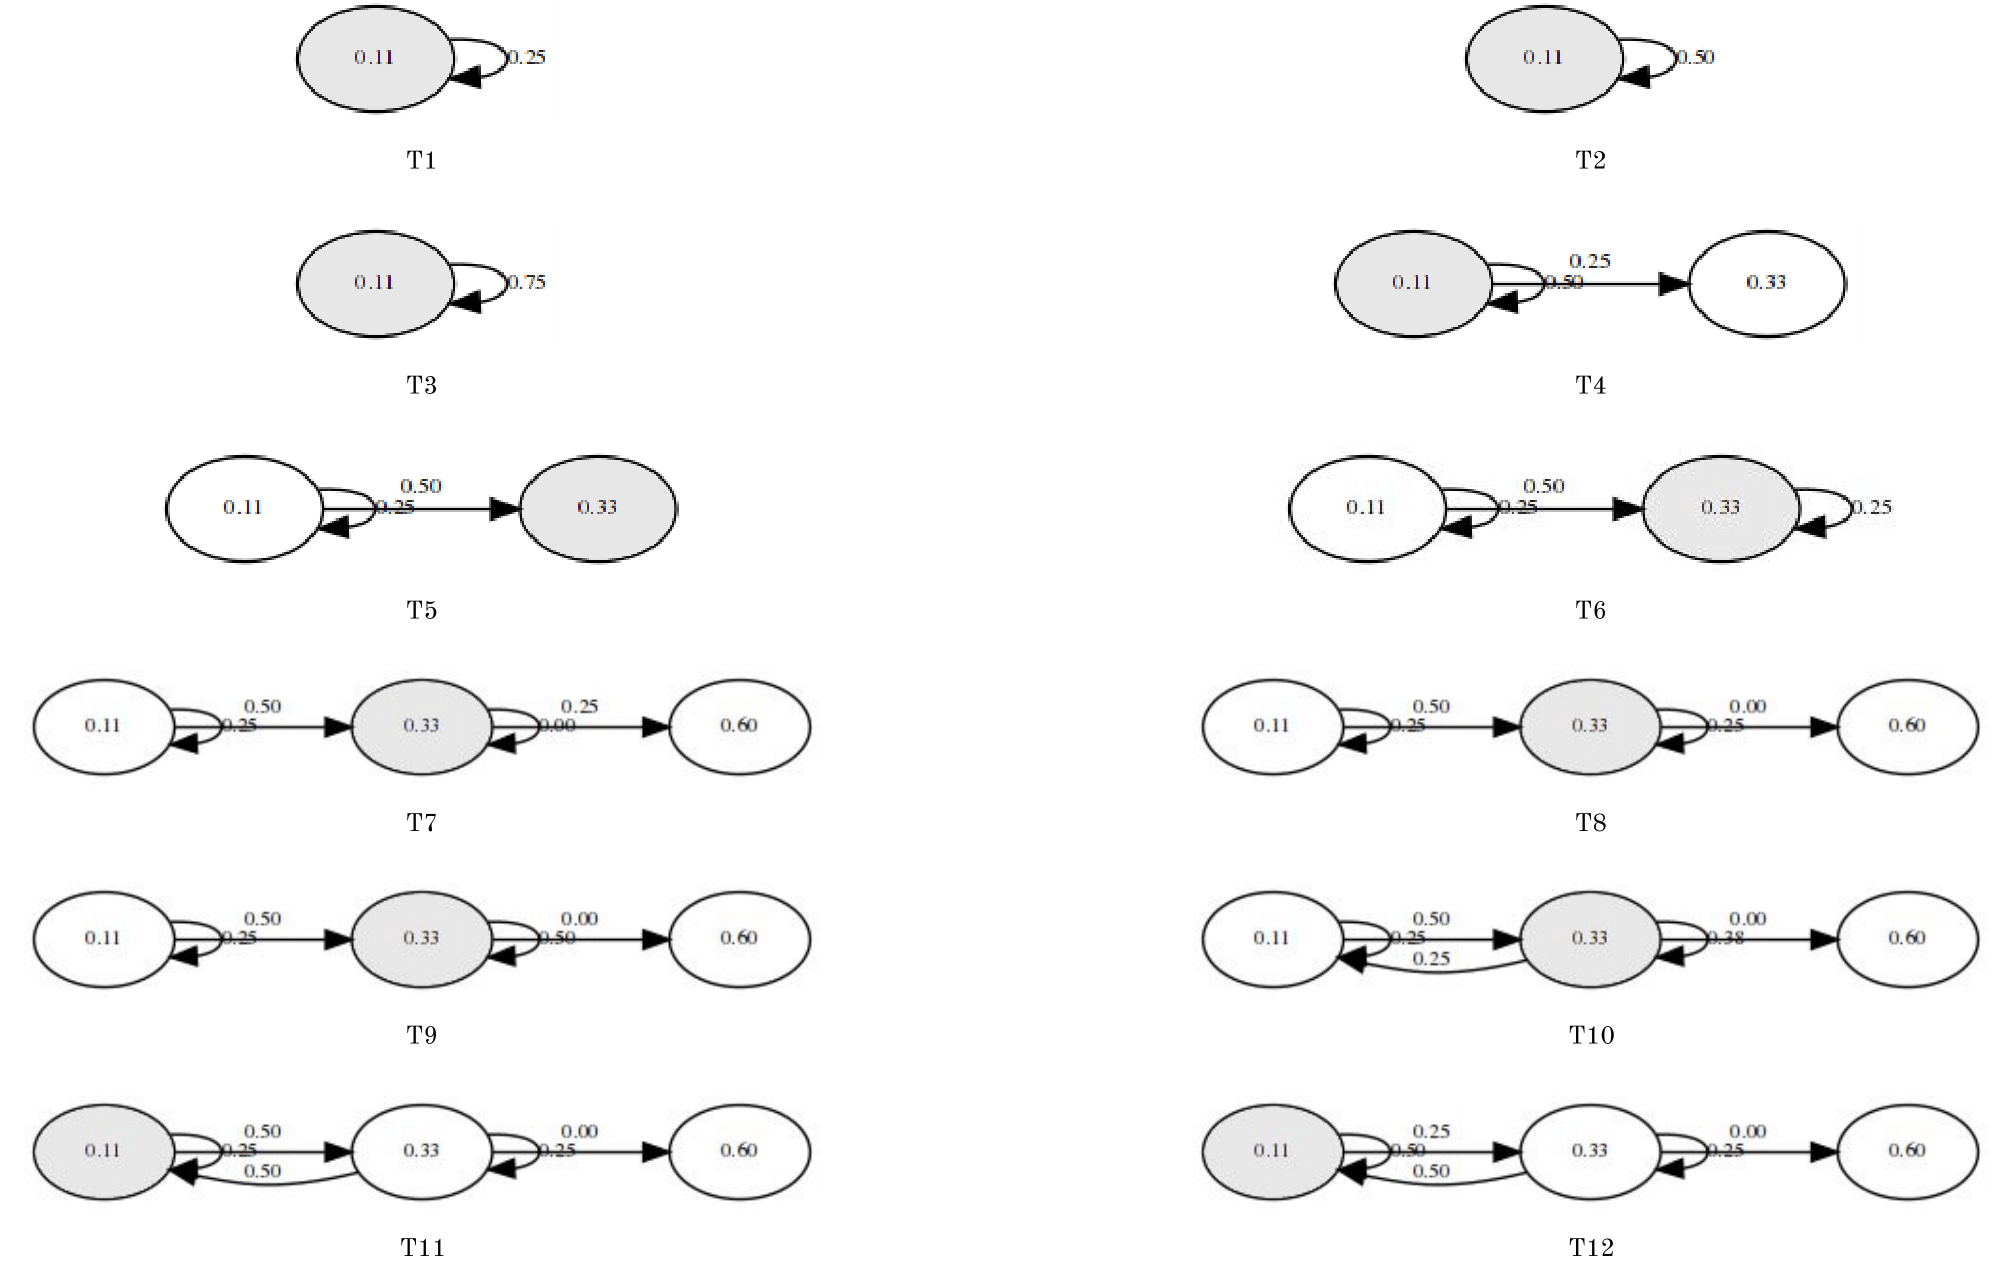
\includegraphics[width=\textwidth]{imagens/evolucao_markov.png}
            \caption{Evolução do modelo markoviano.}
        \label{fig:evolucao_markov}
        \end{center}
    \end{figure}
\end{frame}


\section{Experimentos}


\begin{frame}{Dados Sintéticos}
    \begin{itemize}
        \item O primeiro experimento utilizou dados sintéticos produzidos por versões adaptadas das classes geradoras do MOA.
        \item Foram utilizados $4$ conjuntos de dados, com $2.500$ eventos cada.
        \item Os eventos possuem valores entre $0$ e $1$, com adição de um ruído randômico entre $[-0.1, 0.2]$.
        \item Cada conjunto de dados pode representar até $2$ conceitos distintos.
        \item Cada conceito é composto por $400$ eventos.
    \end{itemize}
\end{frame}

\begin{frame}{Dados Sintéticos}
    \begin{figure}[ht]
        \begin{center}
            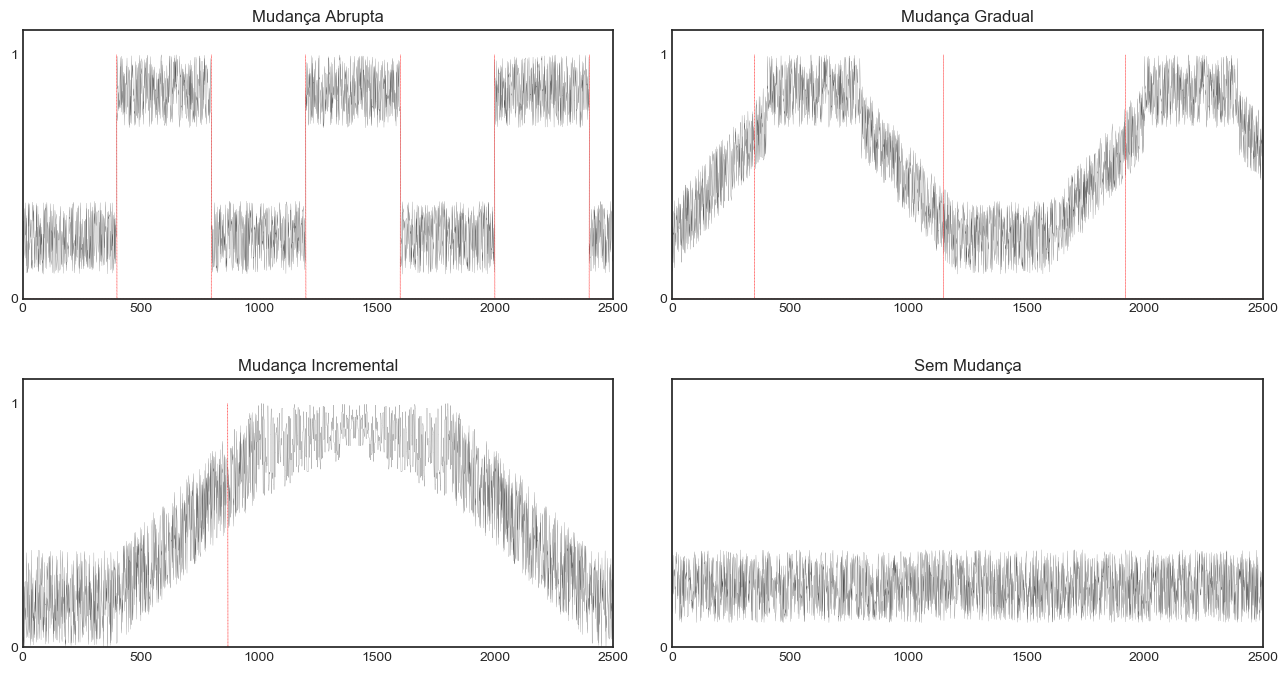
\includegraphics[width=\textwidth]{imagens/conjuntos_dados_sinteticos.png}
            \caption{Representação gráfica dos conjuntos de dados sintéticos.}
            \label{fig:conjuntos_dados_sinteticos}
        \end{center}
    \end{figure}
\end{frame}


\begin{frame}{Dados Sintéticos - Métricas}
    \begin{table}[h]
        \centering
        \caption{Métricas utilizadas na avaliação com dados sintéticos.}
        \label{tbl:indicadores_analisado}
        \begin{tabularx}{\textwidth}{ll}
        \toprule
        Métrica & Observação \\
        \midrule
        TP       &  \textbf{Tempo de Processamento} por instância (média em seg.). \\
        MR       &  \textbf{Mudanças Reais} existentes no conjunto de dados. \\
        VP       &  \textbf{Verdadeiro Positivo}. Quantidade de detecções corretas. \\
        FP       &  \textbf{Falso Positivo}. Quantidade de detecções errôneas. \\
        ATR      &  \textbf{Atraso de detecção}. \\
                 &  Quantidade média de instâncias até a detecção. \\
        \bottomrule
        \end{tabularx}
    \end{table}
\end{frame}

\begin{frame}{Dados Sintéticos -  Sem mudanças de conceito}
    \begin{figure}[t]
        \begin{center}
            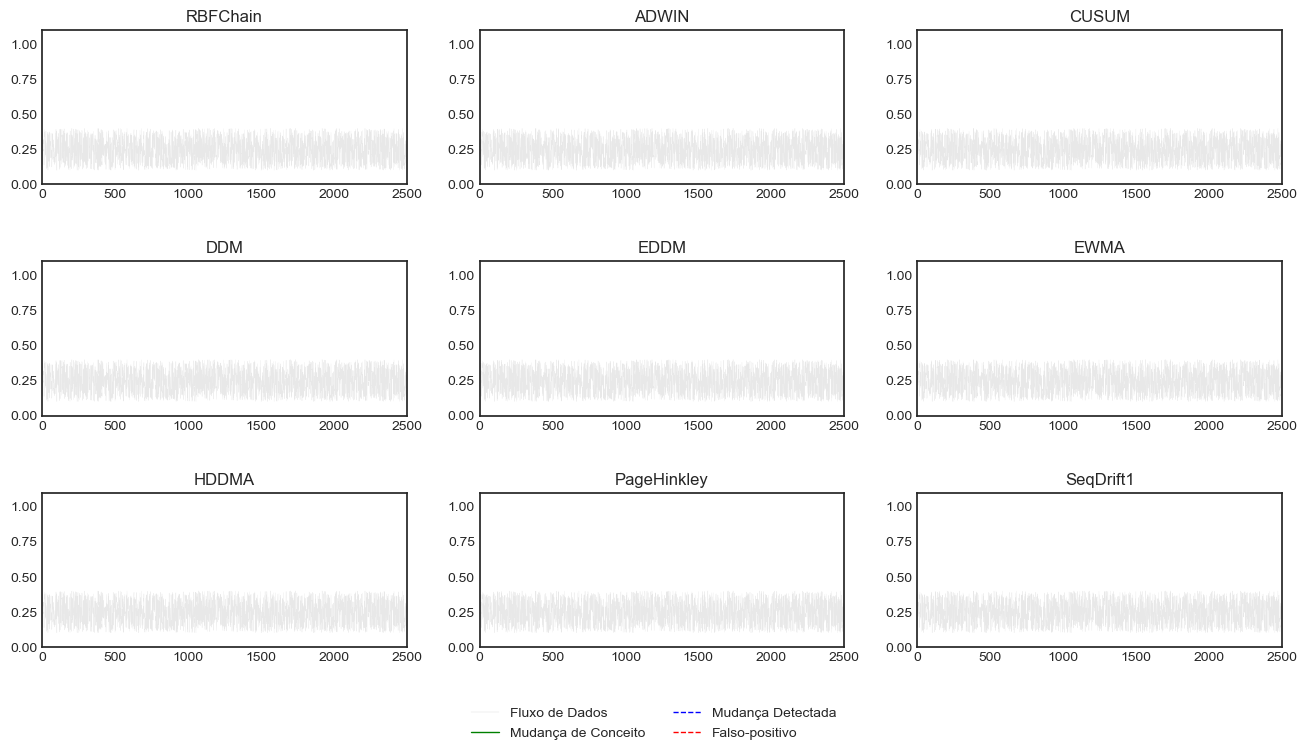
\includegraphics[width=\textwidth]{imagens/nochange.png}
            \caption{Comportamento dos algoritmos para o conjunto de dados sem mudanças de conceito.}
            \label{fig:exp_sem_mudancas}
        \end{center}
    \end{figure}
\end{frame}


\begin{frame}{Dados Sintéticos -  Sem mudanças de conceito}
    \begin{table}[h]
        \centering
        \caption{Resultados dos algoritmos para o conjunto de dados sem mudanças de conceito.}
        \label{tbl:exp1}
        \begin{tabular}{llllll}

        \toprule
        Algoritmo              & TP                     & MR                     & VP                     & FP                     & ATR                    \\
        \midrule
        RBFChain               & \alert{0.013}                  & 0                      & 0                      & 0                      & ---                    \\
        ADWIN                  & 0.025                  & 0                      & 0                      & 0                      & ---                    \\
        CUSUM                  & 0.016                  & 0                      & 0                      & 0                      & ---                    \\
        DDM                    & 0.014                  & 0                      & 0                      & 0                      & ---                    \\
        EDDM                   & \alert{0.013}                  & 0                      & 0                      & 0                      & ---                    \\
        EWMA                   & 0.014                  & 0                      & 0                      & 0                      & ---                    \\
        HDDMA                  & 0.017                  & 0                      & 0                      & 0                      & ---                    \\
        PageHinkley            & 0.015                  & 0                      & 0                      & 0                      & ---                    \\
        SeqDrift1              & 0.017                  & 0                      & 0                      & 0                      & ---                    \\
        \bottomrule

        \end{tabular}
    \end{table}
\end{frame}

\begin{frame}{Dados Sintéticos -  Sem mudanças de conceito}
    \begin{itemize}
        \item Todos algoritmos testados demonstraram tolerância a ruídos e não indicaram nenhum falso positivo.
        \item RBFChain obteve a melhor média em tempo de processamento, juntamente com o EDDM.
    \end{itemize}
\end{frame}

\begin{frame}{Dados Sintéticos -  Mudanças Abruptas}
    \begin{figure}[t]
        \begin{center}
            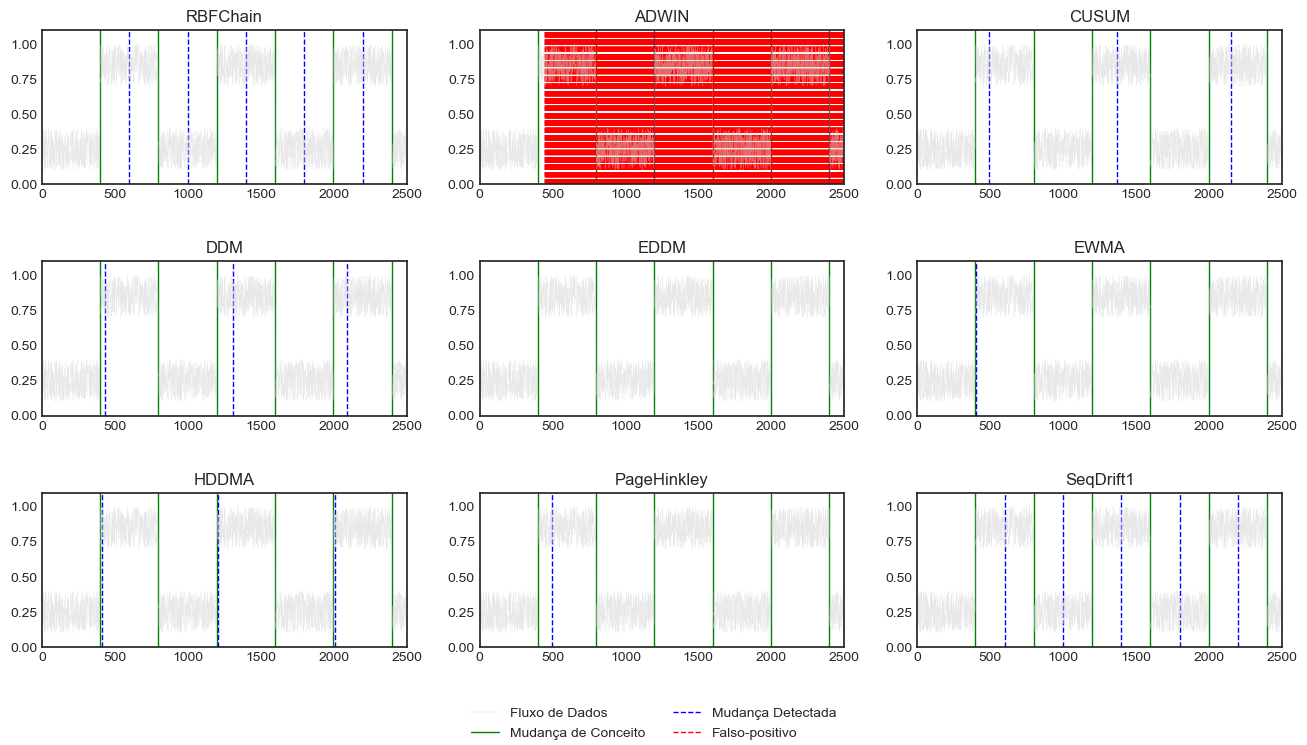
\includegraphics[width=\textwidth]{imagens/abrupt.png}
            \caption{Comportamento dos algoritmos para o conjunto de dados com mudanças de conceito abruptas.}
            \label{fig:exp_abrupta}
        \end{center}
    \end{figure}
\end{frame}

\begin{frame}{Dados Sintéticos -  Mudanças Abruptas}
    \begin{table}[ht]
        \centering
        \caption{Resultados dos algoritmos para o conjunto de dados com mudanças de conceito abruptas.}
        \label{tbl:exp2}
        \begin{tabular}{llllll}

    \toprule
    Algoritmo              & TP                     & MR                     & VP                     & FP                     & ATR                    \\
    \midrule
    RBFChain               & 0.015                  & 6                      & \alert{5}              & 0                      & 166.67                 \\
    ADWIN                  & 0.016                  & 6                      & 6                      & \textcolor{red}{2046}  & 9.00                   \\
    CUSUM                  & 0.021                  & 6                      & 3                      & 0                      & 68.83                  \\
    DDM                    & 0.015                  & 6                      & 3                      & 0                      & 38.83                  \\
    EDDM                   & 0.013                  & 6                      & 0                      & 0                      & ---                    \\
    EWMA                   & 0.014                  & 6                      & 1                      & 0                      & 1.00                   \\
    HDDMA                  & 0.014                  & 6                      & 3                      & 0                      & 10.00                    \\
    PageHinkley            & 0.015                  & 6                      & 1                      & 0                      & 16.17                  \\
    SeqDrift1              & 0.015                  & 6                      & \alert{5}              & 0                      & 167.50                 \\
    \bottomrule

        \end{tabular}
        \end{table}
\end{frame}

\begin{frame}{Dados Sintéticos -  Mudanças Abruptas}
    \begin{itemize}
        \item RBFChain e SeqDrift1 apresentaram as melhores acurácias, identificando 5 das 6 mudanças existentes, sem produzir nenhum falso positivo.
        \item RBFChain apresentou o terceiro melhor tempo de processamento (TP), com uma pequena diferença para o primeiro.
        \item ADWIN se mostrou hipersensível.
    \end{itemize}
\end{frame}

\begin{frame}{Dados Sintéticos -  Mudanças Graduais}
    \begin{figure}[t]
        \begin{center}
            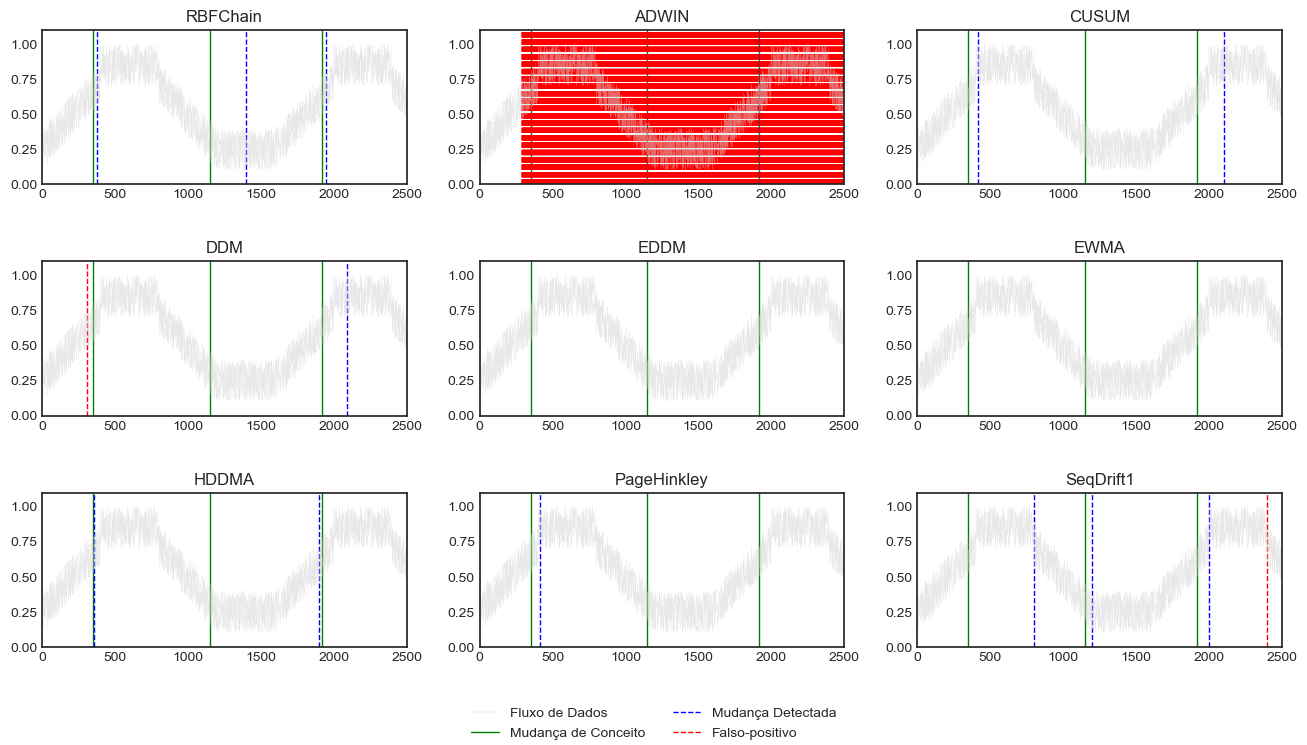
\includegraphics[width=\textwidth]{imagens/gradual.png}
            \caption{Comportamento dos algoritmos para o conjunto de dados com mudanças de conceito graduais.}
            \label{fig:exp_gradual}
        \end{center}
    \end{figure}
\end{frame}

\begin{frame}{Dados Sintéticos -  Mudanças Graduais}
    \begin{table}[ht]
        \centering
        \caption{Resultados dos algoritmos para o conjunto de dados com mudanças de conceito graduais.}
        \label{tbl:exp3}
        \begin{tabular}{llllll}

        \toprule
        Algoritmo              & TP                     & MR                     & VP                     & FP                     & ATR                    \\
        \midrule
        RBFChain               & \alert{0.011}          & 3                      & \alert{3}              & \alert{0}              & \alert{101.00}         \\
        ADWIN                  & 0.020                  & 3                      & 3                      & 2209                   & 1.00                   \\
        CUSUM                  & 0.014                  & 3                      & 2                      & 0                      & 83.33                  \\
        DDM                    & 0.014                  & 3                      & 1                      & 1                      & 58.33                  \\
        EDDM                   & 0.013                  & 3                      & 0                      & 0                      & ---                    \\
        EWMA                   & 0.015                  & 3                      & 0                      & 0                      & ---                    \\
        HDDMA                  & 0.014                  & 3                      & 2                      & 0                      & 100.67                 \\
        PageHinkley            & 0.014                  & 3                      & 1                      & 0                      & 22.33                  \\
        SeqDrift1              & 0.015                  & 3                      & \alert{3}              & \alert{1}              & \alert{194.33}         \\
        \bottomrule


        \end{tabular}
        \end{table}
\end{frame}

\begin{frame}{Dados Sintéticos -  Mudanças Graduais}
    \begin{itemize}
        \item RBFChain obteve a melhor acurácia, identificando todas as três mudanças de conceito, sem produzir falso positivos.
        \item Algoritmo SeqDrift1 apresentou a segunda melhor acurácia, pois também detectou as três mudanças corretamente, entretanto, apresentou um falso positivo e uma taxa de atraso significativamente maior.
        \item RBFChain também apresentou o melhor tempo de processamento.
    \end{itemize}
\end{frame}

\begin{frame}{Dados Sintéticos -  Mudanças Incrementais}
    \begin{figure}[t]
        \begin{center}
            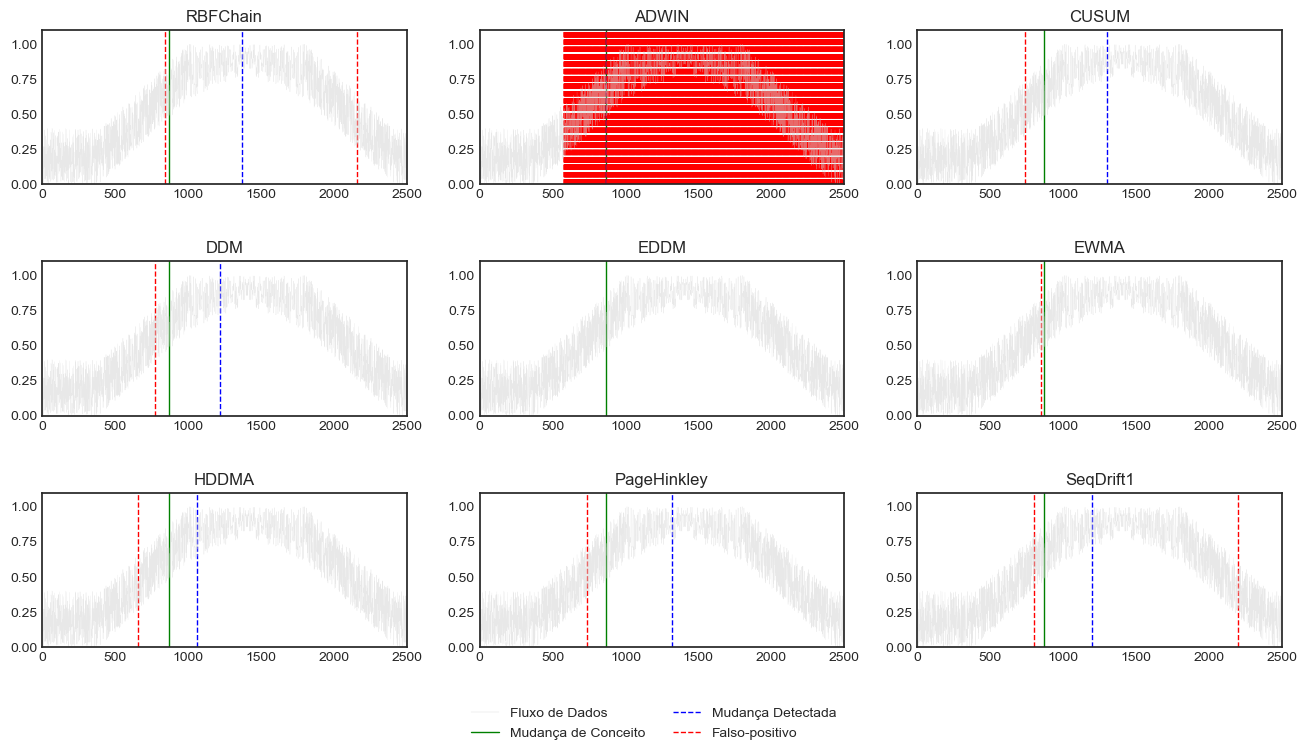
\includegraphics[width=\textwidth]{imagens/incremental.png}
            \caption{Comportamento dos algoritmos para o conjunto de dados com mudanças de conceito incrementais.}
            \label{fig:exp_incremental}
        \end{center}
    \end{figure}
\end{frame}

\begin{frame}{Dados Sintéticos -  Mudanças Incrementais}
    \begin{table}[ht]
        \centering
        \caption{Resultados dos algoritmos para o conjunto de dados com mudanças de conceito incrementais.}
        \label{tbl:exp4}
        \begin{tabular}{llllll}

        \toprule
        Algoritmo              & TP                     & MR                     & VP                     & FP                     & ATR                    \\
        \midrule
        RBFChain               & 0.020                  & 1                      & 1                      & 2                      & 501.00                 \\
        ADWIN                  & 0.017                  & 1                      & 1                      & 1923                   & 1.00                   \\
        CUSUM                  & 0.014                  & 1                      & 1                      & 1                      & 434.00                 \\
        DDM                    & 0.014                  & 1                      & 1                      & 1                      & 349.00                 \\
        EDDM                   & 0.013                  & 1                      & 0                      & 0                      & ---                    \\
        EWMA                   & 0.016                  & 1                      & 0                      & 1                      & ---                    \\
        HDDMA                  & 0.014                  & 1                      & 1                      & 1                      & 213.00                    \\
        PageHinkley            & 0.014                  & 1                      & 1                      & 1                      & 449.00                 \\
        SeqDrift1              & 0.016                  & 1                      & 1                      & 2                      & 331.00                 \\
        \bottomrule

        \end{tabular}
        \end{table}
\end{frame}

\begin{frame}{Dados Sintéticos -  Mudanças Incrementais}
    \begin{itemize}
        \item A mudança de conceito incremental representa uma dificuldade, pois todos algoritmos que detectaram a mudança existente também produziram falso positivos.
        \item RBFChain e SeqDrift1, que apresentaram os melhores resultados nos testes anteriores, tiveram a pior acurácia, pois emitiram dois falsos positivo cada.
        \item Teste considerado inconclusivo, ressaltando a necessidade de uma investigação mais detalhada sobre a detecção de mudanças de conceito incrementais.
    \end{itemize}
\end{frame}

\begin{frame}{Dados Reais - Identificação de fixações e sacadas}
    \begin{itemize}
        \item Dados de monitoramento ocular têm sido utilizados por uma quantidade significativa de pesquisas, em diferentes áreas do conhecimento.
        \item Os dados brutos coletados precisam ser identificados em eventos, como fixações e sacadas, para serem analisados.
        \item O processo de identificação é realizado por algoritmos. Entretanto, nenhum algoritmo existente na literatura permitir identificar eventos em tempo de execução.
        \item Para superar esta limitação, empregamos o RBFChain na identificação de fixações e sacadas.
    \end{itemize}
\end{frame}

\begin{frame}{Dados Reais - Identificação de fixações e sacadas}
    \begin{figure}[H]
        \begin{center}
            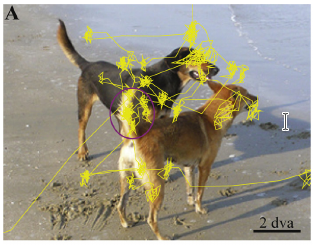
\includegraphics[scale=1]{imagens/exemplo_fixacao_e_sacadas.png}
            \caption{Exemplo de identificação de fixações e sacadas. Fonte: \cite{KONIG2014121}.}
            \label{fig:exemplo_fixacoes_e_sacadas}
        \end{center}
    \end{figure}
\end{frame}

\begin{frame}{Dados Reais - Identificação de fixações e sacadas}
    \begin{itemize}
        \item O experimento utilizou dados de dois macacos-prego (Dede e Juju) produzidos e cedidos pelo Instituto do Cérebro (UFRN).
        \item Cada conjunto de dados possui $6.200$ eventos, que indicam a localização do olhar ao longo do tempo $(x, y)$.
        \item O RBFChain foi ligeiramente adaptado para analisar a alternância (sacadas) e a continuidade (fixações) dos conceitos.
        \item Os resultados foram validados através de métricas de classificação, utilizando os resultados do algoritmo ClusterFix \cite{KONIG2014121} como rótulos.
    \end{itemize}
\end{frame}

\begin{frame}{Dados Reais - Identificação de fixações e sacadas -  Trajetórias}
    \begin{columns}
        \begin{column}{0.48\textwidth}
            \begin{figure}[H]
                \begin{center}
                    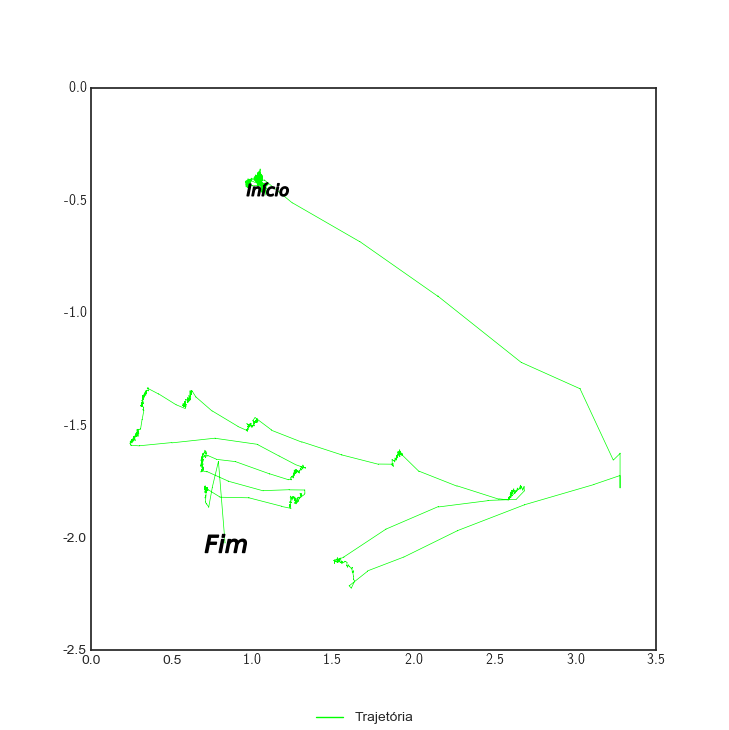
\includegraphics[scale=0.25]{imagens/trajetoria_dede.png}
                    \caption{Trajetória \textit{Dede}.}
                \end{center}
            \end{figure}
        \end{column}
        \begin{column}{0.48\textwidth}
            \begin{figure}[H]
                \begin{center}
                    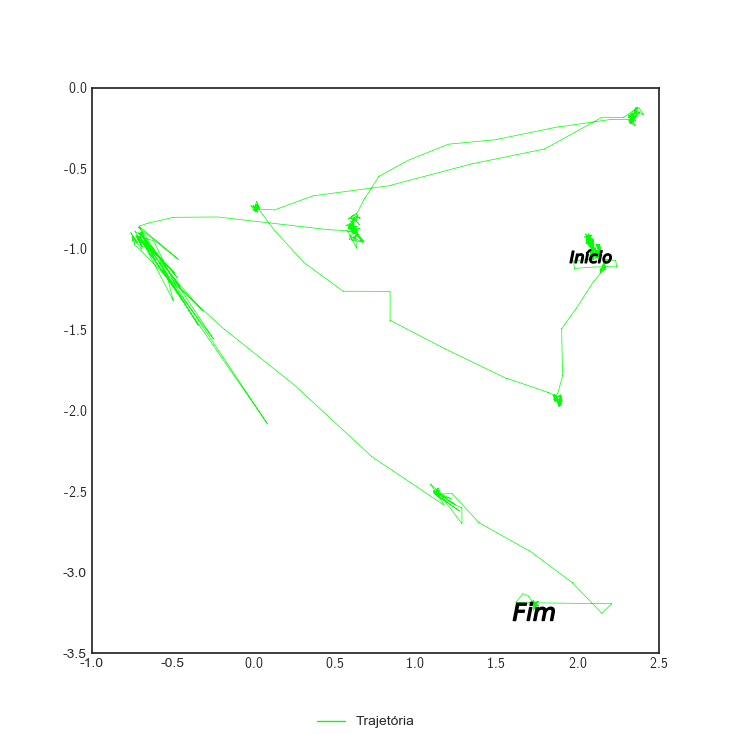
\includegraphics[scale=0.25]{imagens/trajetoria_juju.png}
                    \caption{Trajetória \textit{Juju}.}
                \end{center}
            \end{figure}
        \end{column}
    \end{columns}
\end{frame}

\begin{frame}{Dados Reais - Identificação de fixações e sacadas -  Métricas}
    \begin{table}[h]
        \centering
        \caption{Métricas utilizadas na avaliação com dados reais.}
        \label{tbl:metricas_rbfchain}
        \begin{tabularx}{\textwidth}{lX}
        \toprule
        Métrica  & Observação \\
        \midrule
        QP       &  \textbf{Quantidade de Pontos} analisados. \\
        AC       &  \textbf{Acurácia}.  \\
                 & Fração de fixações e sacadas identificadas corretamente. \\

        PR       &  \textbf{Precisão}.  \\
                 & Fração das fixações identificadas pelo algoritmo corretamente.  \\

        RE       &  \textbf{\textit{Recall}}.  \\
                 & Fração das fixações existentes (rotuladas) que também foram identificadas pelo algoritmo.  \\

        \bottomrule
        \end{tabularx}
        \end{table}
\end{frame}

\begin{frame}{Dados Reais - Identificação de fixações e sacadas -  Dede}
    \begin{columns}
        \begin{column}{0.48\textwidth}
            \begin{figure}[H]
                \begin{center}
                    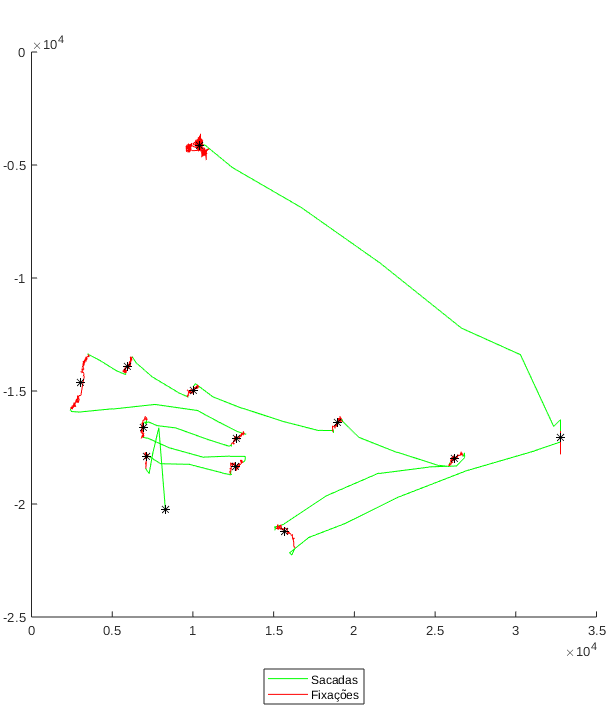
\includegraphics[scale=0.25]{imagens/dede_clusterfix.png}
                    \caption{ClusterFix - \textit{Dede}.}
                \end{center}
            \end{figure}
        \end{column}
        \begin{column}{0.48\textwidth}
            \begin{figure}[H]
                \begin{center}
                    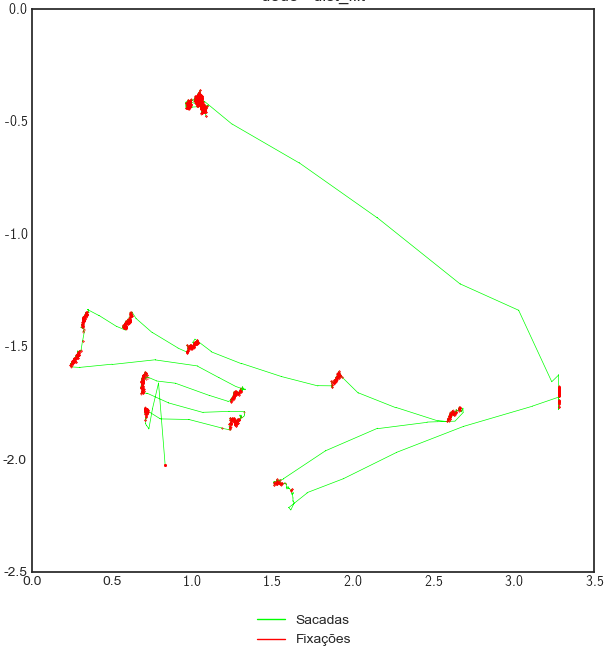
\includegraphics[scale=0.28]{imagens/dede_rbfchain.png}
                    \caption{RBFChain - \textit{Dede}.}
                \end{center}
            \end{figure}
        \end{column}
    \end{columns}
\end{frame}

\begin{frame}{Dados Reais - Identificação de fixações e sacadas -  Dede}
    \begin{table}[ht!]
        \centering
        \caption{Resultados para o conjunto de dados \textit{Dede}.}
        \label{tbl:dede}
        \begin{tabular}{llll}

        \toprule
        QT              & AC                     & PR                     & RE         \\
        \midrule
        $6.200$         & $0.87$                 & $0.98$                 & $0.88$      \\
        \bottomrule

        \end{tabular}
    \end{table}

    \begin{itemize}
        \item \alert{$87\%$} das fixações e sacadas identificadas pelo RBFChain tiveram a mesma classificação pelo ClusterFix.
        \item \alert{$98\%$} das fixações identificadas pelo RBFChain tiveram a mesma classificação pelo ClusterFix.
        \item \alert{$88\%$} das fixações identificadas pelo ClusterFix também foram identificadas pelo RBFChain.
    \end{itemize}
\end{frame}

\begin{frame}{Dados Reais - Identificação de fixações e sacadas -  Juju}
    \begin{columns}
        \begin{column}{0.48\textwidth}
            \begin{figure}[H]
                \begin{center}
                    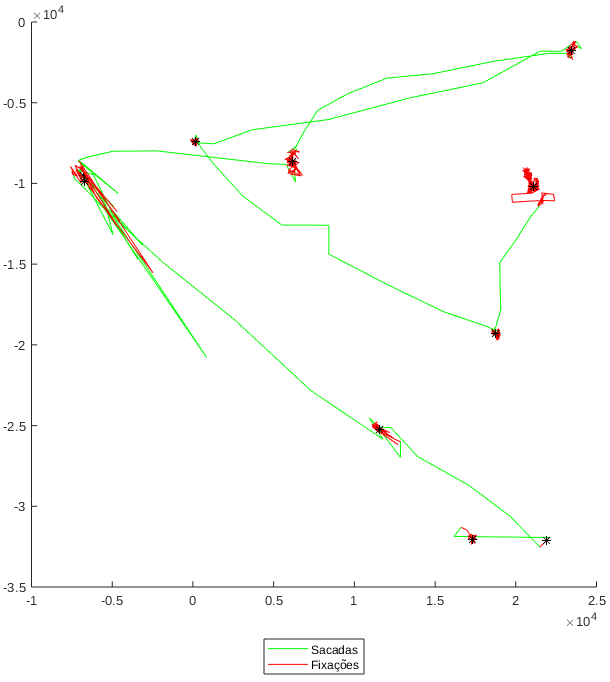
\includegraphics[scale=0.25]{imagens/juju_clusterfix.png}
                    \caption{ClusterFix - \textit{Juju}.}
                \end{center}
            \end{figure}
        \end{column}
        \begin{column}{0.48\textwidth}
            \begin{figure}[H]
                \begin{center}
                    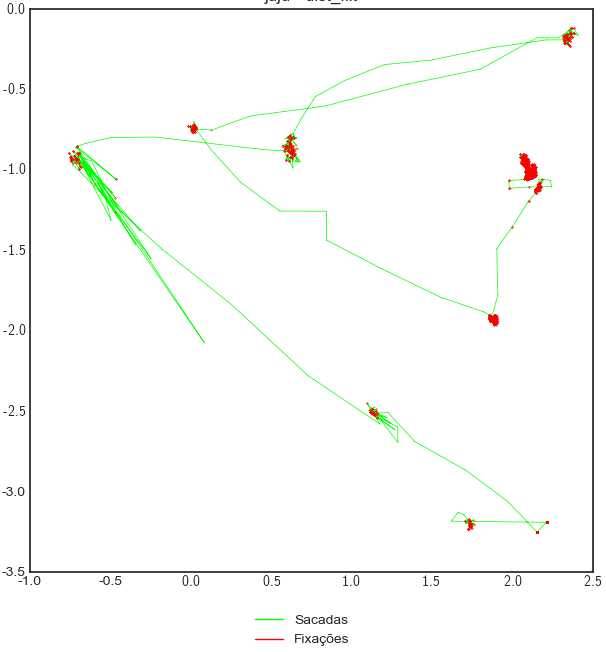
\includegraphics[scale=0.28]{imagens/juju_rbfchain.png}
                    \caption{RBFChain - \textit{Juju}.}
                \end{center}
            \end{figure}
        \end{column}
    \end{columns}
\end{frame}

\begin{frame}{Dados Reais - Identificação de fixações e sacadas -  Juju}
    \begin{table}[ht!]
        \centering
        \caption{Resultados para o conjunto de dados \textit{Juju}.}
        \label{tbl:juju}
        \begin{tabular}{llll}

        \toprule
        QT              & AC                     & PR                     & RE      \\
        \midrule
        $6.200$         & $0.82$                 & $0.98$                 & $0.83$      \\
        \bottomrule

        \end{tabular}
    \end{table}

    \begin{itemize}
        \item \alert{$82\%$} das fixações e sacadas identificadas pelo RBFChain tiveram a mesma classificação pelo ClusterFix.
        \item \alert{$98\%$} das fixações identificadas pelo RBFChain tiveram a mesma classificação pelo ClusterFix.
        \item \alert{$83\%$} das fixações identificadas pelo ClusterFix também foram identificadas pelo RBFChain.
    \end{itemize}
\end{frame}

\section{Conclusões e Trabalhos Futuros}

\begin{frame}{Conclusões}
    \begin{itemize}
        \item Novo método de detecção de mudanças de conceito, capaz de detectar mudanças em tempo de execução, de forma computacionalmente eficiente e independente de rótulos;
        \item Novo método para identificação de fixações e sacadas em tempo de execução, com acurácia equivalente ao estado da arte.
    \end{itemize}
\end{frame}

\begin{frame}{Trabalhos Futuros}
    \begin{itemize}
        \item Desenvolvimento de novas estratégias para o cálculo dos parâmetros.
        \item Criação de novas bases de dados experimentais.
        \item Investigação aprofundada sobre a detecção de mudanças incrementais.
    \end{itemize}
\end{frame}

\begin{frame}[allowframebreaks]{Referências}

  \bibliography{slides}
  \bibliographystyle{abbrv}

\end{frame}

\end{document}
